\begin{frame}{}
  Avec un.e partenaire, déterminez le mot qui ne correspond pas aux autres pour chaque numéro.
  \begin{columns}
    \column{0.5\textwidth}
      \begin{enumerate}
        \item HLM, immeuble, \textcolor<2->{red}{trottoir}, gratte-ciel, pavillon
        \item chic, \textcolor<4->{red}{délabré}, spacieux, élégant, rénové
        \item \textcolor<6->{red}{mendiant}, centre-ville, quartier, périphérie, banlieue
        \item flâner, faire du lèche-vitrines, se promener, \textcolor<8->{red}{louer}, se balader
      \end{enumerate}
    \column{0.5\textwidth}
      \begin{minipage}[c][0.75\textheight]{\linewidth}
        \begin{center}
          \only<2>{
            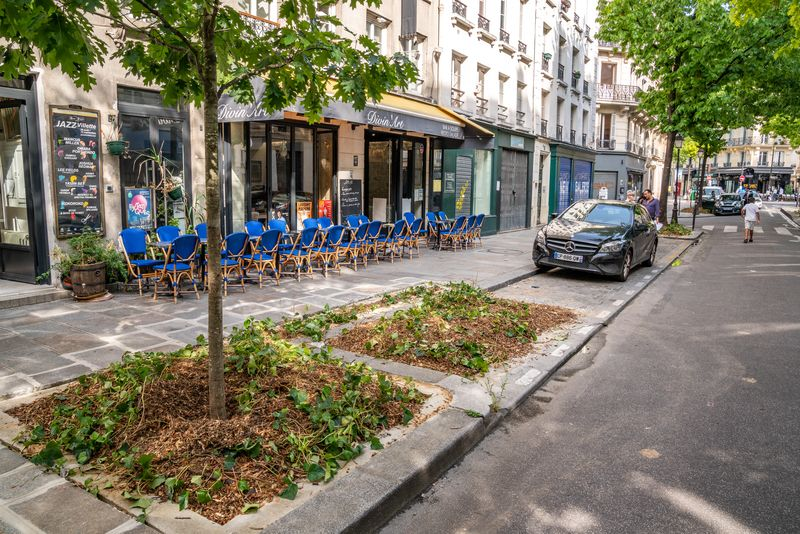
\includegraphics[scale=0.2]{trottoir_paris.jpg} \\
            Paris
          }
          \only<4>{
            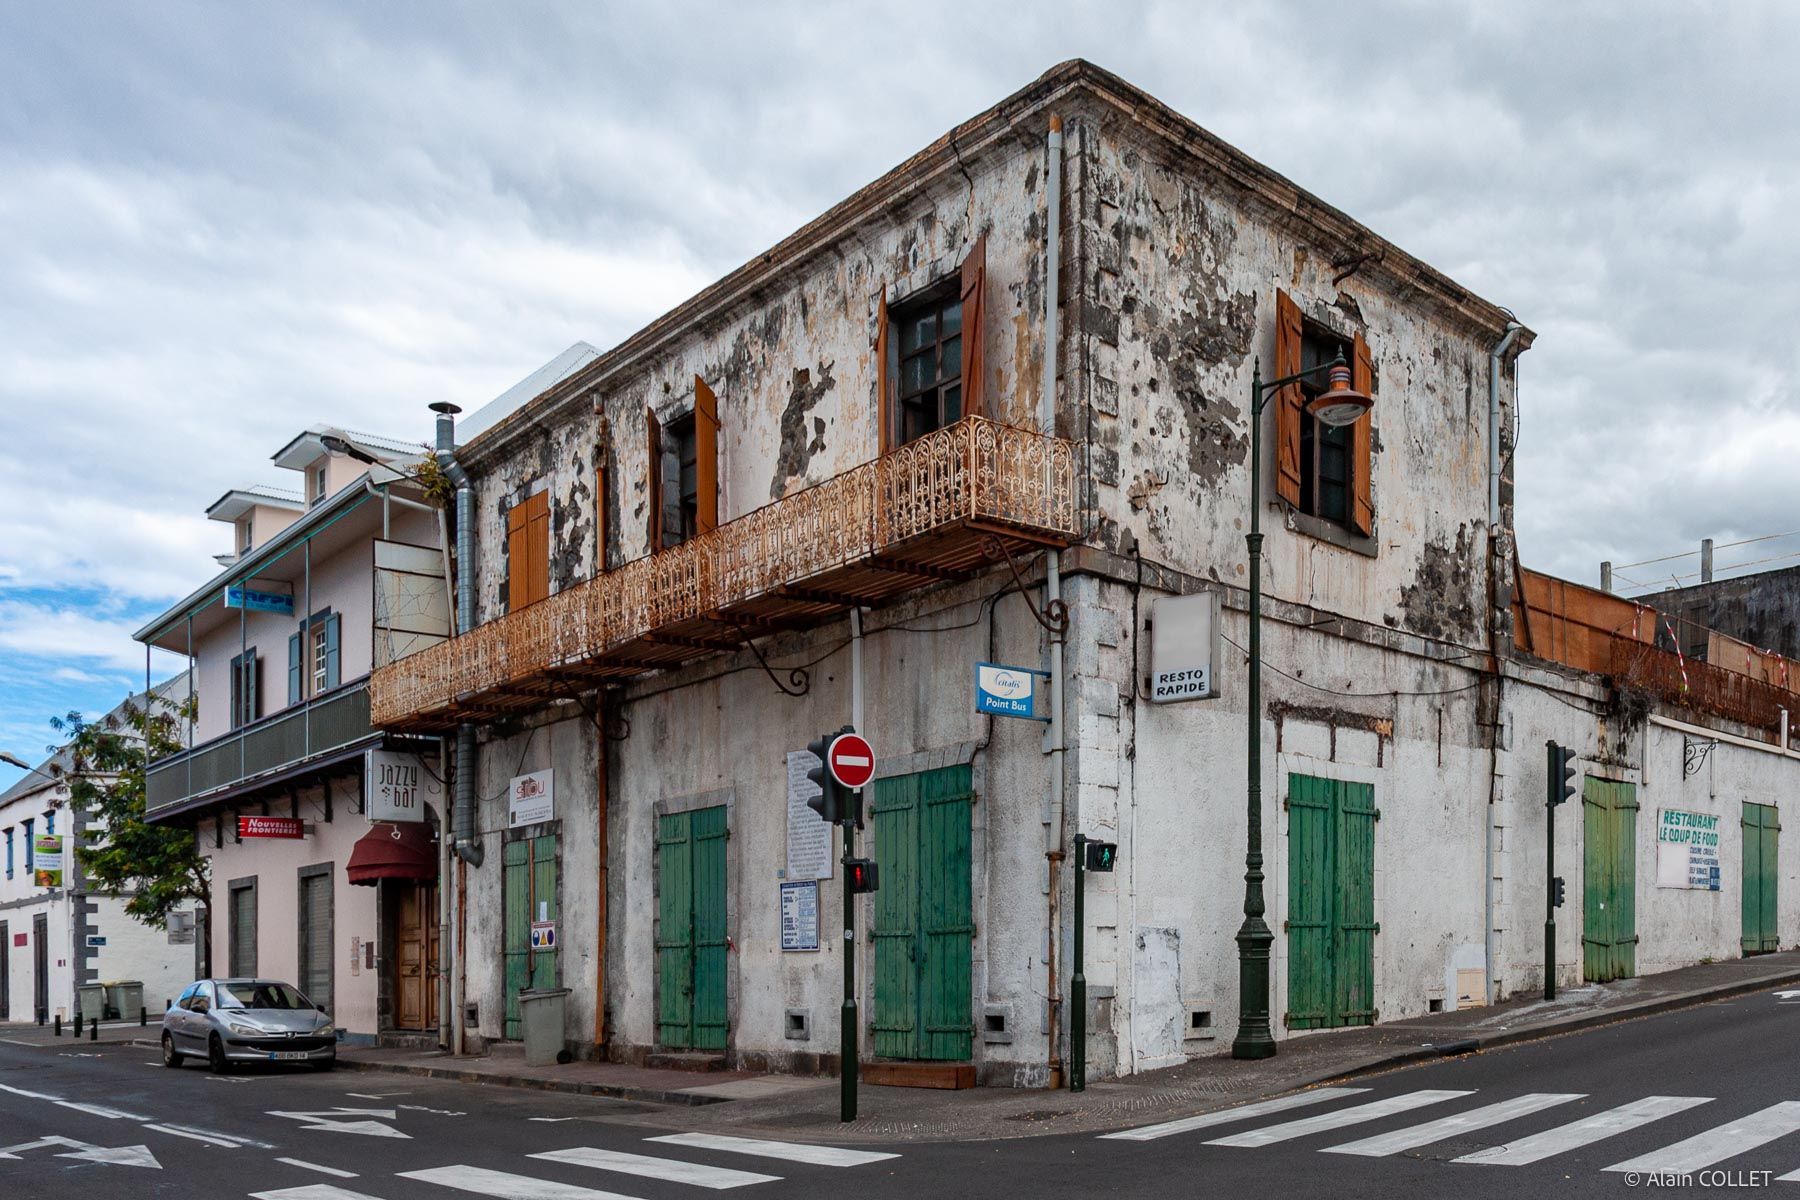
\includegraphics[scale=0.3]{saint-denis_reunion.jpg} \\
            Saint-Denis, La Réunion
          }
          \only<6>{
            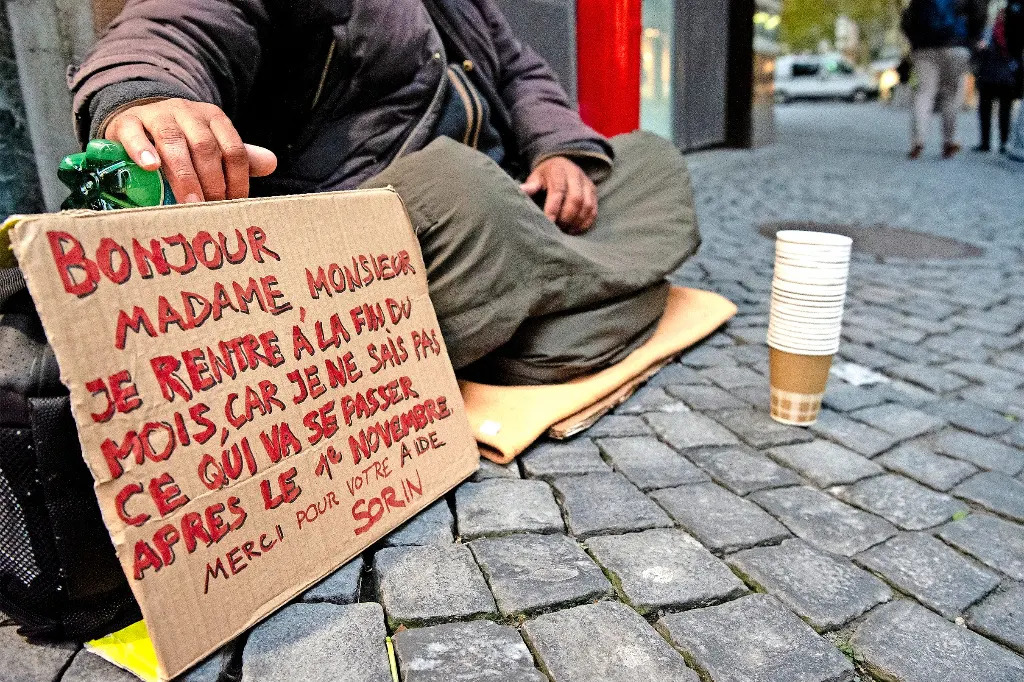
\includegraphics[scale=0.16]{mendiant.jpg}
          }
          \only<8>{
            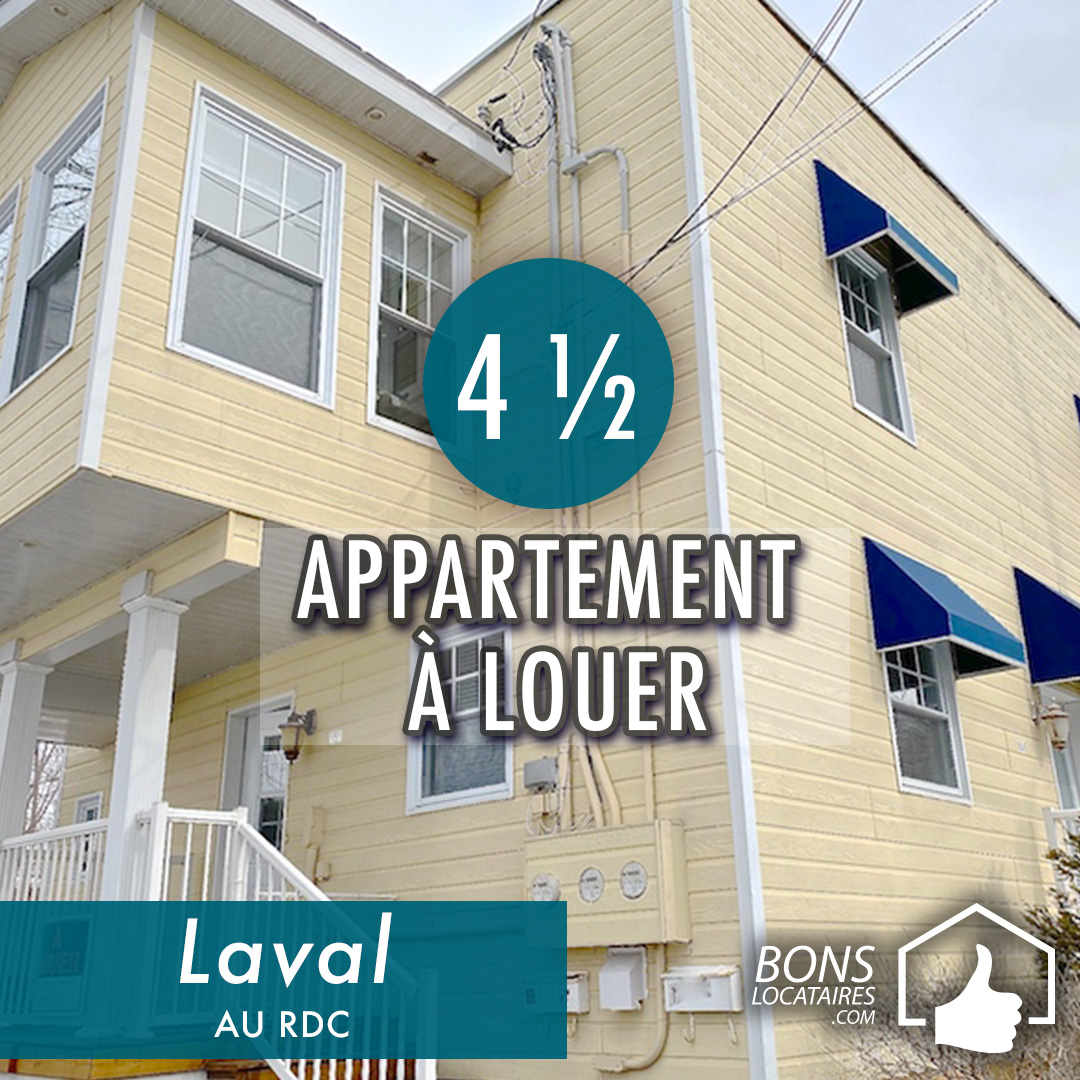
\includegraphics[scale=0.14]{louer_laval.jpg} \\
            Laval, le Québec
          }
        \end{center}
      \end{minipage}
  \end{columns}
\end{frame}